\documentclass{homework}
\usepackage[utf8]{inputenc}
\usepackage{xspace,color,url,listings,graphicx,float,amsmath,amssymb,braket,subcaption}
\graphicspath{{./graphs/}} %location of images

\lstset{commentstyle=\color{red},keywordstyle=\color{black},
showstringspaces=false}
\lstnewenvironment{rc}[1][]{\lstset{language=R}}{}
\newcommand{\ri}[1]{\lstinline{#1}}  %% Short for 'R inline'

\lstset{language=R}             % Set R to default language

\newcommand{\hwname}{Shara Duong, Charles Colgan, Josh Borders}
\newcommand{\hwnum}{2}

\newcommand{\hwtype}{Homework}
\newcommand{\hwclass}{MATH 6350}

\begin{document}

\maketitle

Shara Duong: Wrote and edited code. Edited text of document.\\
Charles Colgan: Wrote and edited code. Edited text of document. Created tables and figures.\\
Josh Borders: Wrote text of the document. \\


\textbf{PART ZERO:} We chose Vladimir, Ebrima, and Bitstream Vera (hereafter, Bitstream) for our fonts. After discarding null observations, n(Vladimir) = 244, n(Ebrima) = 1723, and n(Bitstream) = 2296. We then combined these observations into a single data frame.

Each observation is described by a row of 400 features, the level of grayness in each pixel. We standardized each feature, x$_j$, by re-centering about the mean and dividing by the standard deviation, such that:
\begin{align*}
    sx_j = \frac{x_j-\bar{x_j}}{\sigma_{x_j}} 
\end{align*}
This makes our classification method, K nearest neighbors(KNN), more reliable, since it is dependent on distance; in other words, no one feature has an out-sized effect on the classifier before the analysis begins. 

These "standardized" observations are used for the rest of the exercises. We computed a correlation matrix of the features, dimension 400 x 400, and extracted the ten highest values, as seen in Table \ref{tab:Table 1}. Feature pair r11c2 and r12c2 have close to a 95-percent association, while r7c1 and r8c1 have an approximately 92-percent association. These high correlation values imply that pixels right beside each other have similar gray levels, which is understandable.
\begin{table}[H]
    \centering
    \begin{tabular}{c|c|c}
    row&col&cor\\\hline
  r11c2&r12c2&0.942\\
  r12c2&r13c2&0.937\\
   r9c1&r10c1&0.932\\
  r11c1&r12c1&0.931\\
  r12c1&r13c1&0.931\\
 r12c18&r13c18&0.927\\
   r9c0&r10c0&0.927\\
 r11c17&r12c17&0.924\\
   r9c2&r10c2&0.923\\
   r7c1&r8c1&0.922
    \end{tabular}
    \caption{The 10 highest correlation values}
    \label{tab:Table 1}
\end{table}
Next we randomly selected 20\% of the standardized observations for each class for use as our test set, leaving the other 80\% to train our classifier. Importantly, we kept proportional representation of each font class in our test and train sets, as this prevents biasing classifiers or veracity thereof.

\question
KNN classifies on the basis that nearby cases are similarly classed. To do this, the distance from any given case to the k cases nearest to it is measured and is then used to attempt a classification. k=12 was chosen for our initial KNN classification, the confusion matrix for which is shown in Table \ref{tab:Table 2}. Our classifier correctly predicted \textbf{90.7 percent} of the cases in the training set, and it correctly predicted \textbf{89.8 percent} of the cases in the test set, with a \textbf{global accuracy of 90.26 percent}. This performance is reasonably good, especially for a first choice of k.
\begin{table}[h]
    \centering
    \begin{tabular}{c|cc}
         &Train&Test \\\hline
         Train&0.907&0.093 \\
         Test&0.102&0.898
    \end{tabular}
    \caption{Confusion matrix for k=12}
    \label{tab:Table 2}
\end{table}
\question
We computed the percentage of correctly classified cases for the test set using different values for k, from 1 to 100. The graph of this is shown in Figure \ref{fig:Figure 1}. It demonstrates that the classifier likely works best when k=1, as the percentage of correctly classified observations is roughly 94 percent. From this point, as k increases, our accuracy on the testing set decreases. It may, therefore, be wise to investigate \textbf{k in a range from (1, 10)}, but k any greater than that will lead to a poorly performing classifier. The spike at k=100 is misleading, as the percentage of correctly classified observations for k=100 is actually 84 percent. It must be considered an aberration of the plot.

\begin{figure}[h]
    \centering
    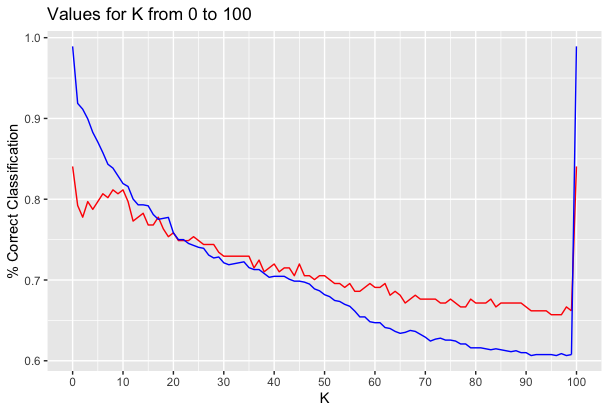
\includegraphics[width=13cm]{graphs/Krange.png}
    \caption{Test Set Accuracy for K in Range (1, 100). Red is training set, blue is test set.}
    \label{fig:Figure 1}
\end{figure}

\question
We further isolated the region where k is chosen between 1 and 10, which is shown in Figure \ref{fig:Figure 2}. It once again indicates that \textbf{k=1} is likely the best choice of k for our classifier.

\begin{figure}[h]
    \centering
    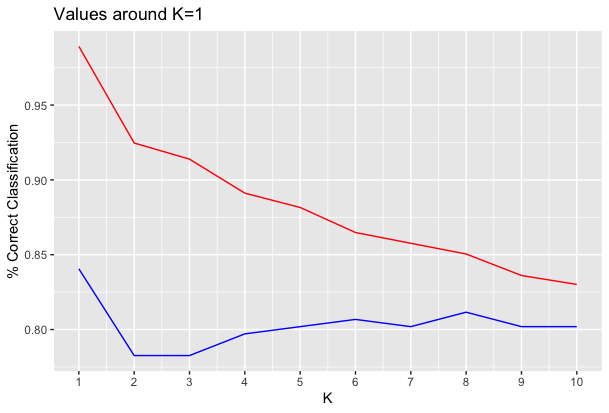
\includegraphics[width=13cm]{graphs/Kbest.png}
    \caption{Test Set Accuracy for K in Range (1, 10). Red is training set, blue is test set.}
    \label{fig:Figure 2}
\end{figure}

\question
Choosing k=1, we classified on the training data and then predicted the true classification for the testing data. The results for the training and testing accuracy, test1. The classifier correctly classified almost all of the training data, with a global accuracy of 99.91 percent, but struggled on the testing data. While it correctly predicted roughly 98 percent of Bitstream cases and 90 percent of Ebrima, it fared worse with classifying Vladimir, only predicting the correct instance 83 percent of the time. This resulted in a global accuracy of 93.77 percent. True Vladimir cases were classified as Ebrima 15 percent of the time, and as Bitstream 2 percent of the time.

\begin{table}[h]
    \centering
        \begin{tabular}{c|ccc}
         &BITSTREAM&EBRIMA&VLADIMIR\\\hline
         BITSTREAM&1.000&0.000&0.000\\
         EBRIMA&0.000&1.000&0.000\\
         VLADIMIR&0.00&0.015&0.985
    \end{tabular}
    \caption{Training confusion Matrix for k=1}
    \label{tab:Table 3}
\end{table}
\begin{table}[h]
    \centering
    \begin{tabular}{c|ccc}
         &BITSTREAM&EBRIMA&VLADIMIR\\\hline
         BITSTREAM&0.976&0.022&0.002\\
         EBRIMA&0.093&0.901&0.006\\
         VLADIMIR&0.021&0.146&0.833
    \end{tabular}
    \caption{Test confusion matrix for k=1}
    \label{tab:Table 4}
\end{table}

\question
The 90\% confidence intervals for the accurate classification from the train confusion matrix are as follows: (1.000,1.000) for Bitstream, (1.000,1.000) for  Ebrima, and (0.970, 0.999) for Vladimir.\\
For the test confusion matrix, the 90\% confidence intervals were:
(0.964, 0.988) for Bitstream, (0.875, 0.928) for Ebrima, and (0.745, 0.922) for Vladimir.\\ 
We are 90 percent confident that the true accuracy of our classifier for the respective fonts are contained in the above ranges.

For each font, the confidence interval is more narrow for the training set than it is for the test set, and there is little overlap between the two. The intervals being nearly disjoint may suggest that the true frequency of correct classification is higher for the training set than it is for the test set.\\ 
Comparing the estimated frequencies, we have the 90\% confidence interval of their differences to be: (0.012, 0.035) for Bitstream, (0.072, 0.125) for Ebrima, and (0.062, 0.241) for Vladimir. Because none of these intervals contain 0, we reject the hypothesis that the true percentages for both sets are close to each other.

\question
We split our original train and test data into four sections and then took a subsection (PACK) of 100 values from the first ten values of each index. We ran KNN with k=1 on each PACK. For the first set of 100 features, Pack1, our classifier returned an accuracy on its corresponding testing set of \textbf{92.2 percent}. 

\question
Likewise, we applied KNN with k=1 on the remaining PACKs. The accuracy of prediction for each PACK's corresponding testing set was 0.912, 0.905, and 0.934 for PACK2, PACK3, and PACK4 respectively. Thus, k=1 correctly predicted 91.2 percent of observations in Pack2, 90.5 percent of observations in Pack3, and 93.4 percent of observations in Pack4.

\question
We then generated weights (w1,w2,w3,w4) for each PACK using their performance on their corresponding test sets. As such, the features in Pack 1, 2, and 4 were weighted more heavily than those features in Pack 3, though the difference is not drastic. We then normalized the weights so their sums equaled one. These normalized weights are 0.251, 0.249, 0.246, and 0.254 for w1, w2, w3, and w4 respectively.

We then weighted each feature by its appropriate weight and applied KNN with k=1. The global accuracy was \textbf{93.89 percent}, and the confusion matrix is as in Table \ref{tab:Table 5}.
\begin{table}[H]
    \centering
    \begin{tabular}{c|ccc}
         &BITSTREAM&EBRIMA&VLADIMIR\\\hline
         BITSTREAM&0.976&0.022&0.002\\
         EBRIMA&0.090&0.904&0.006\\
         VLADIMIR&0.021&0.146&0.833
    \end{tabular}
    \caption{Test confusion matrix for weighted k=1}
    \label{tab:Table 5}
\end{table}
\textbf{Conclusion:} Our k=1 classifier using weighted distances was slightly more accurate than the non-weighted version, performing 0.12\% better on the test set. The weighted classifier was more accurate in predicting the Ebrima font, but not significantly more accurate (roughly 3\% points). This could be an instance of over-fitting on the part of the classifier. The weighted and unweighted classifiers were nearly identical in their predictions of the Bitstream and Vladimir fonts. In sum, the weighted classifier was more accurate, but not by much.

\newpage
\lstinputlisting{code.R}
\end{document}
